
\section{Instrumentación para espectrometría de fluorescencia}

Para caracterizar la respuesta óptica de una sustancia, Generally, one wishes to record both excitation and emission spectra.
the go-to scientific instrument for this measurements is an spectrofluorimeter

\subsection{¿Qué es un espectrofluorímetro? (cap 2 lako)}

A spectrofluorometer enables steady-state intensity measurements such as wavelength scans, time-based ex- periments, synchronous scans, and polarization of luminescence materials aiding research across various sci-entific disciplines including chemistry, biochemistry, pharmacology, environmental science, materials science,and biomedical research. 
The goal of a spectrometer is to get the emission and excitation spectrums of a sample.
For that it has to be able to illuminate a sample with multiple different wavelengths, and record the sample reaction for multiple different wavelengths too.

Figure 2.1 shows a schematic diagram of a general-purpose spectrofluorometer.
It shows all key components to fulfill its purpose
Such lamps are generally useful because of their high intensity at all wavelengths ranging upward from 250 nm. 
The instrument shown is equippedwith monochromators to select both the excitation and emission wavelengths.
monochromators are usually motorized to allow automatic scanning of wavelength.
. This selected excitation light is then focused onto the sampl
The sample luminescence, which usually has a longer wavelength than the excitation light, is then filtered by the emission monochromator.
The light left then arrives at a detector, usally a photomuyltiplier tube PMT, which is a sensitive detector that converts photons into an electric current
spectrofluorometers and all its components use different techniques to decrease stray light light of wavelengths different from the chosen wavelength), like 90degree angle from excitation and emission arm, sealed tight box covered with non-reflective black paint
the pmt signal is then usually processed by electronics, and then digitized and ananlyzed with a PC. 
This PC also orchestrates the monochromators and the acquisition, while providing the user a way to adjust parameters of interest and facilitate data visualization and analysis
usually, aditional components are added in the light path to study different properties of the sample, like shutters, polarizers, beam splitters and other optics elements.



\begin{enumerate}
    \item que mide un espectrofluorimetro?
    \item cuales son sus componentes?
    \item que variables puede controlar?
\end{enumerate}

\begin{figure}[btp]
     \centering
     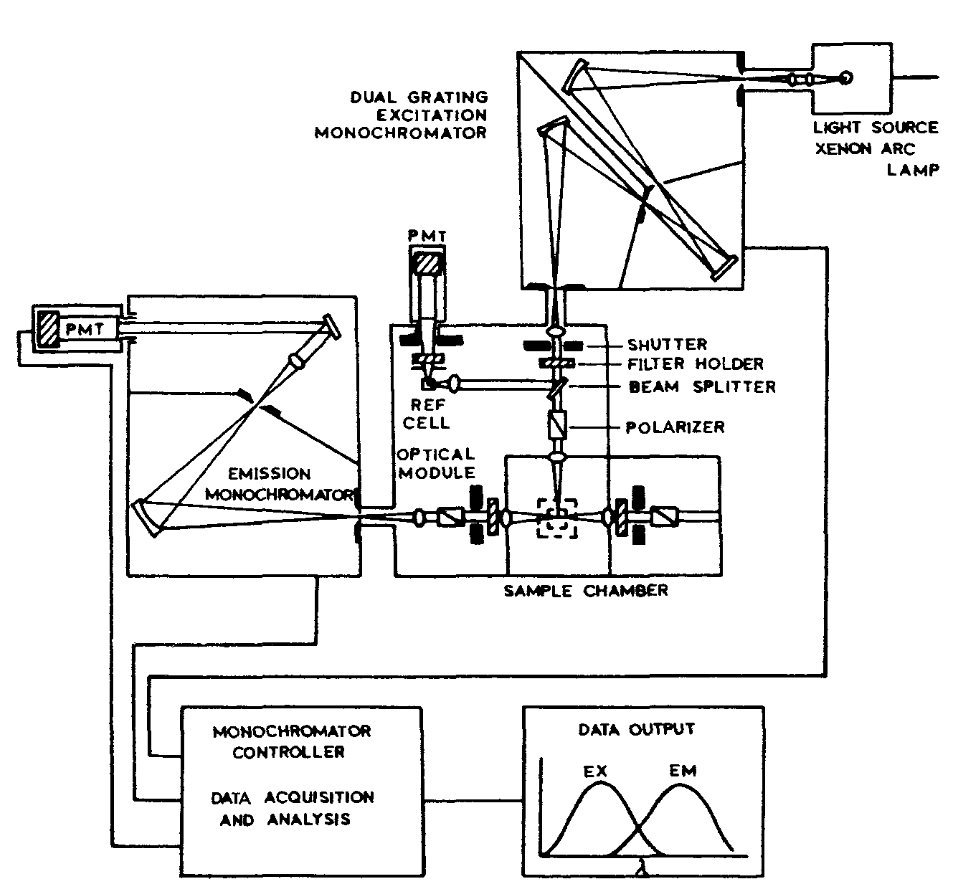
\includegraphics[width=\textwidth]{spectrometer_diagram_lako.png}
     \caption{
    \textbf{Representacioń esquemática de un espectrofluorímetro}
    (\textbf{A}) Diagram of the Horiba PTI QuantaMaster hardware. Red arrows represent motors and limit switch connectors, black is BNC, blue is USB and orange represents a fiber optic. The path that light takes inside the spectrometer is represented in thick blue arrows. 
    (\textbf{B}) and (\textbf{C}) Representation of the old and new instrumental control module respectively.
    (\textbf{D}) Representation of the raw signal measured from the PMT detector.
    (\textbf{E}) Spectrum of the sample constructed from the raw signals measured at each wavelength.
    }
     \label{fig:spec_diagram_lako}
\end{figure}

\subsection{Epectrofluirimetros en argentina y obsolescencia}

espectrofluorimetros disponibles para hacer exp en exactas - sus problemas.

problema no particular de espectrofluorimetria. instrumentos componentes centrales de la investigación científica. obsolescencia de instrumentos: se hecha a perder financiamiento y no se pueden estudiar areas. Intervenir instrumentos closed source para mejorarlos y open source.

alternativa open source para instrumentación. Herramientas open source en general para hacer ciencia e instrumentación.

esta parte de la tesis explica la renovación del horibapti quantamster400


\subsection{Espectrofluorímetro HoribaPTI QuantaMaster 400}

serie horiba quantamaster. frecuencia de aparición en exactas y arg en general, baratos, etc. quizás mencionar lo de stefani

componentes de funcionamiento: conectores originales, lampara, monocromadores, chamber, pmt, especificaciones

software de control: felix gx, capacidades fundamentales y deficiencias

que falta para caracterizar ucnps? time-consuming experiments, operación, medición de tiempos de vida, etc.

\begin{figure}[btp]
     \centering
     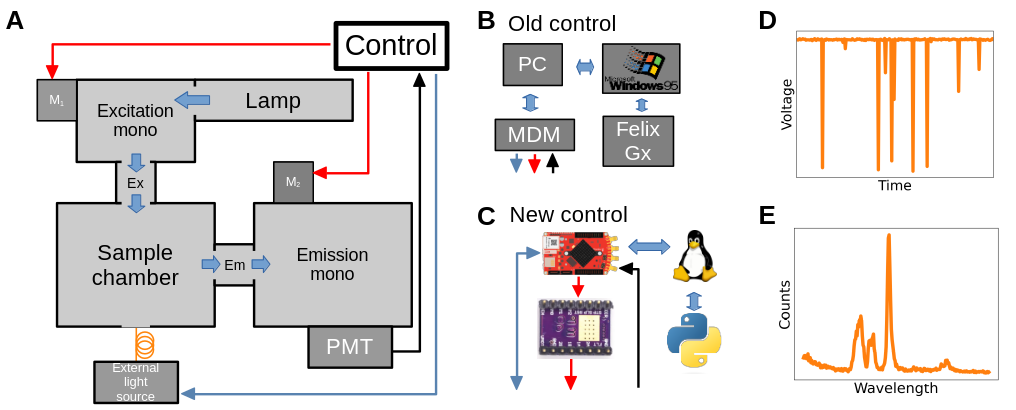
\includegraphics[width=\textwidth]{refurbishment-diagram.png}
     \caption{
    \textbf{Schematic representation of the spectrofluorometer}
    (\textbf{A}) Diagram of the Horiba PTI QuantaMaster hardware. Red arrows represent motors and limit switch connectors, black is BNC, blue is USB and orange represents a fiber optic. The path that light takes inside the spectrometer is represented in thick blue arrows. 
    (\textbf{B}) and (\textbf{C}) Representation of the old and new instrumental control module respectively.
    (\textbf{D}) Representation of the raw signal measured from the PMT detector.
    (\textbf{E}) Spectrum of the sample constructed from the raw signals measured at each wavelength.
    }
     \label{fig:ref-diagram}
\end{figure}

\begin{figure}[h]
     \centering
     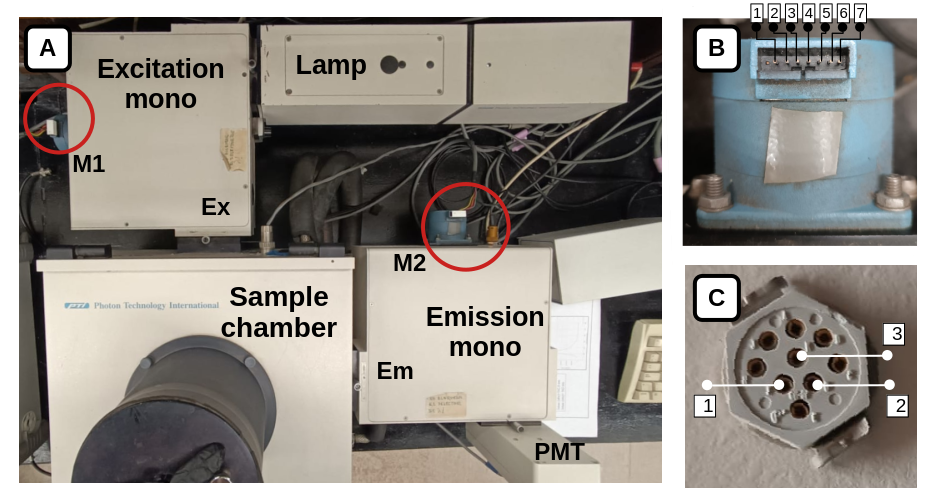
\includegraphics[width=0.9\textwidth]{hardware.png}
     \caption{\textbf{Horiba PTI QuantaMaster 400 picture}. \todo{maybe pasar a apéndice} (\textbf{A}) Picture of the whole spectrometer. Circled in red the monochromators' motors and limit switches. (\textbf{B}) Stepper motors pin diagram. The only used pins for the refurbished version are 1 and 7, and 3 and 5, which correspond to each motor winding respectively. (\textbf{C}) Limit switches pin diagram.}
     \label{fig:hardware}
\end{figure}


\section{Renovación de HoribaPTI QuantaMaster 400}
\subsection{Hardware \todo{quizás es al pedo diferenciar entre hw y sw}}


Qué reemplazamos y con qué nos quedasmos, especificaciones finales

\begin{figure}[h]
     \centering
     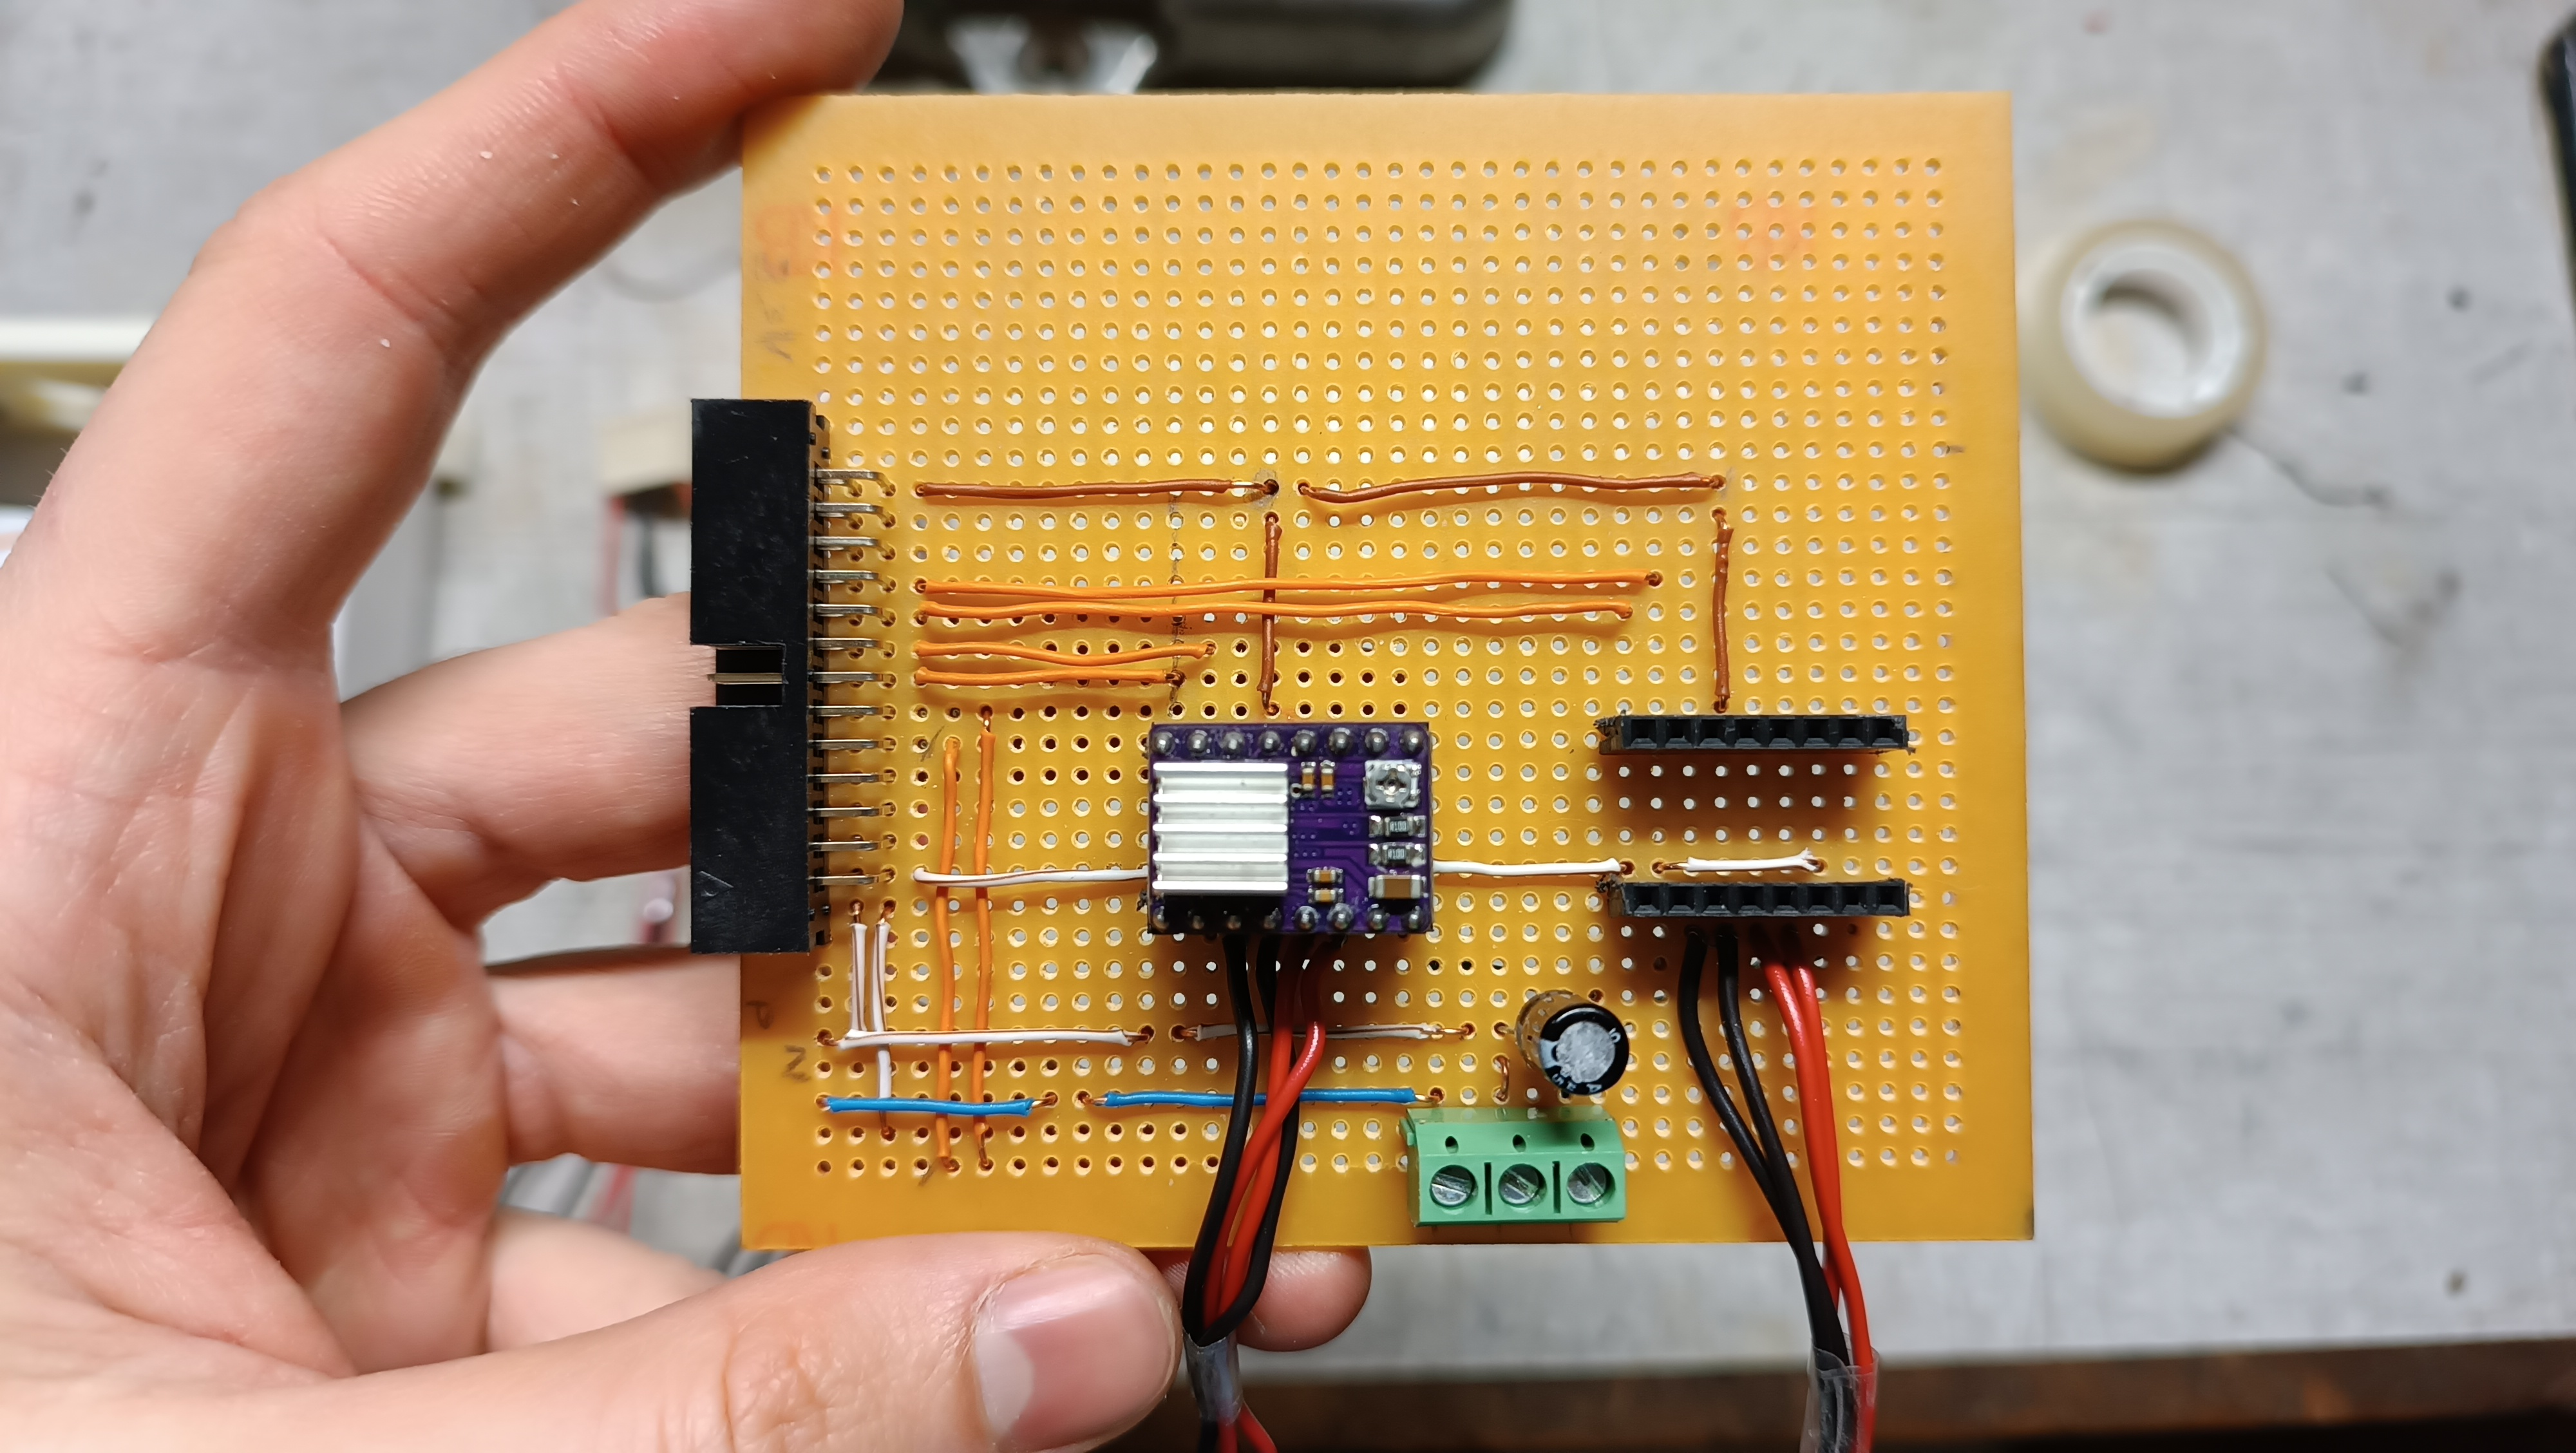
\includegraphics[width=0.9\textwidth]{placa.jpg}
     \caption{\textbf{Horiba PTI QuantaMaster 400 picture}. \todo{maybe pasar a apéndice} (\textbf{A}) Picture of the whole spectrometer. Circled in red the monochromators' motors and limit switches. (\textbf{B}) Stepper motors pin diagram. The only used pins for the refurbished version are 1 and 7, and 3 and 5, which correspond to each motor winding respectively. (\textbf{C}) Limit switches pin diagram.}
     \label{fig:placa}
\end{figure}

\begin{figure}[h]
     \centering
     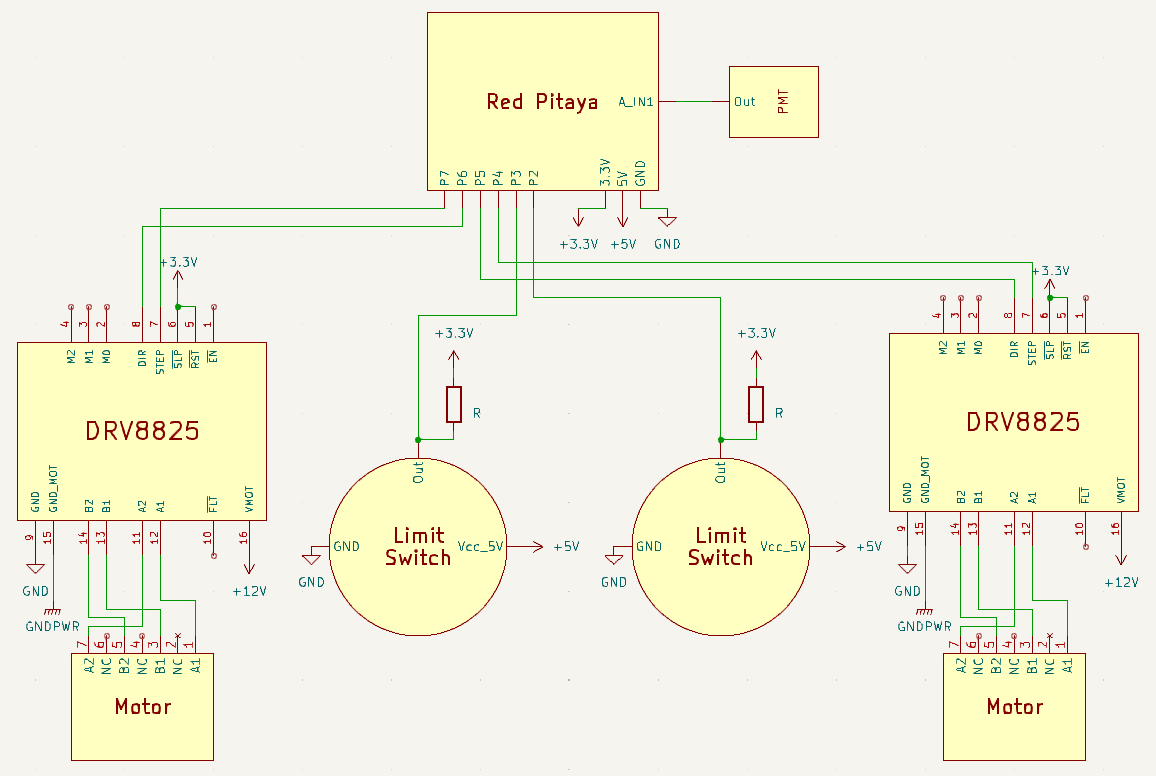
\includegraphics[width=.65\textwidth]{schematic.png}
     \caption{\textbf{Connection diagram}.
     }
     \label{fig:schematic}
\end{figure}

\subsection{Software}

capacidades del software 

Jerarquía de clases API para desacoplar. Extensión del software: sirve para espectrofluorímetro genérico siempre y cuando tengas motor por pasos y pmt.

quien cuenta los picos, (mencionar que hay analisis de picos más adelante)

Modos de uso, API GUI (capacidades, más detallado en apéndice).

\begin{figure}[h]
     \centering
     \caption{\textbf{Structure of the software}. Each element of the software is ordered from high level (\textbf{top}) to low level (\textbf{bottom}). Inside the dashed line black box In yellow, the two ways the end user can interact with the software. In orange, the refurbished instrument API classes. In red, the RP's hardware API.}
     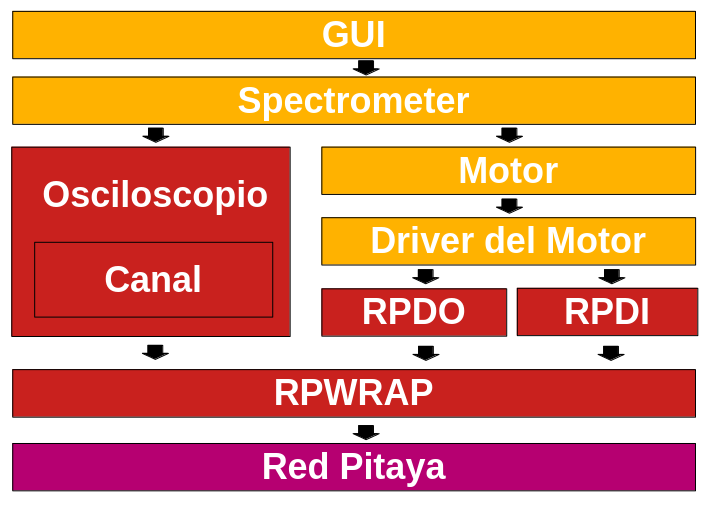
\includegraphics[scale=0.3]{software-diagram.png}
     \label{fig:code}
\end{figure}


\section{Expansión de Horiba PTI QuantaMaster 400 - Medición de tiempos de vida}

introduccion a medicion de tiempos de vida

\subsection{Hardware}

Excitación con laser pulsado. Control de potencia y duty cycle. funcionamiento del trigger. el resto ya lo puede hacer la RP

\subsection{Software}

explicar que es lo mismo que antes salvo que se usa el trigger.

Explicar funcionamiento de las pantallas y offsets
